The recurrence obtained with the analytical solution in \equref{eq:solution} is the following (\equref{eq:recurrent-system}):
\[
  \v{T}_{i+1} = \m{K}_i \: \v{T}_i + \m{B}_i \: \v{P}_i
\]
Given the initial temperature $\v{T}_0$, it can be applied to perform the TTA. Our experiments show that, since intervals $\Delta t_i$ have the same length and matrices $\m{K}_i$ and $\m{B}_i$ become constant, this approach produces a significant performance improvement compared to iterative solutions of ODEs, e.g., the fourth-order Runge-Kutta method used in HotSpot. The same observation is made in \cite{thiele2011}.

The TTA using the analytical technique given in \equref{eq:recurrent-system} can be employed to approximate the SSDTP by applying it over successive application periods, as shown in \secref{sec:hotspot-iterative-solution}. Since each iteration, with this approach, is much faster than with HotSpot, it will significantly speed up the SSDTP calculation. However, the number of required iterations is similar to the case when HotSpot is used (see \figref{fig:hotspot-error}), still keeping the computational process slow (\secref{sec:results-ssdtp}).
\begin{figure}[t]
  \centering
  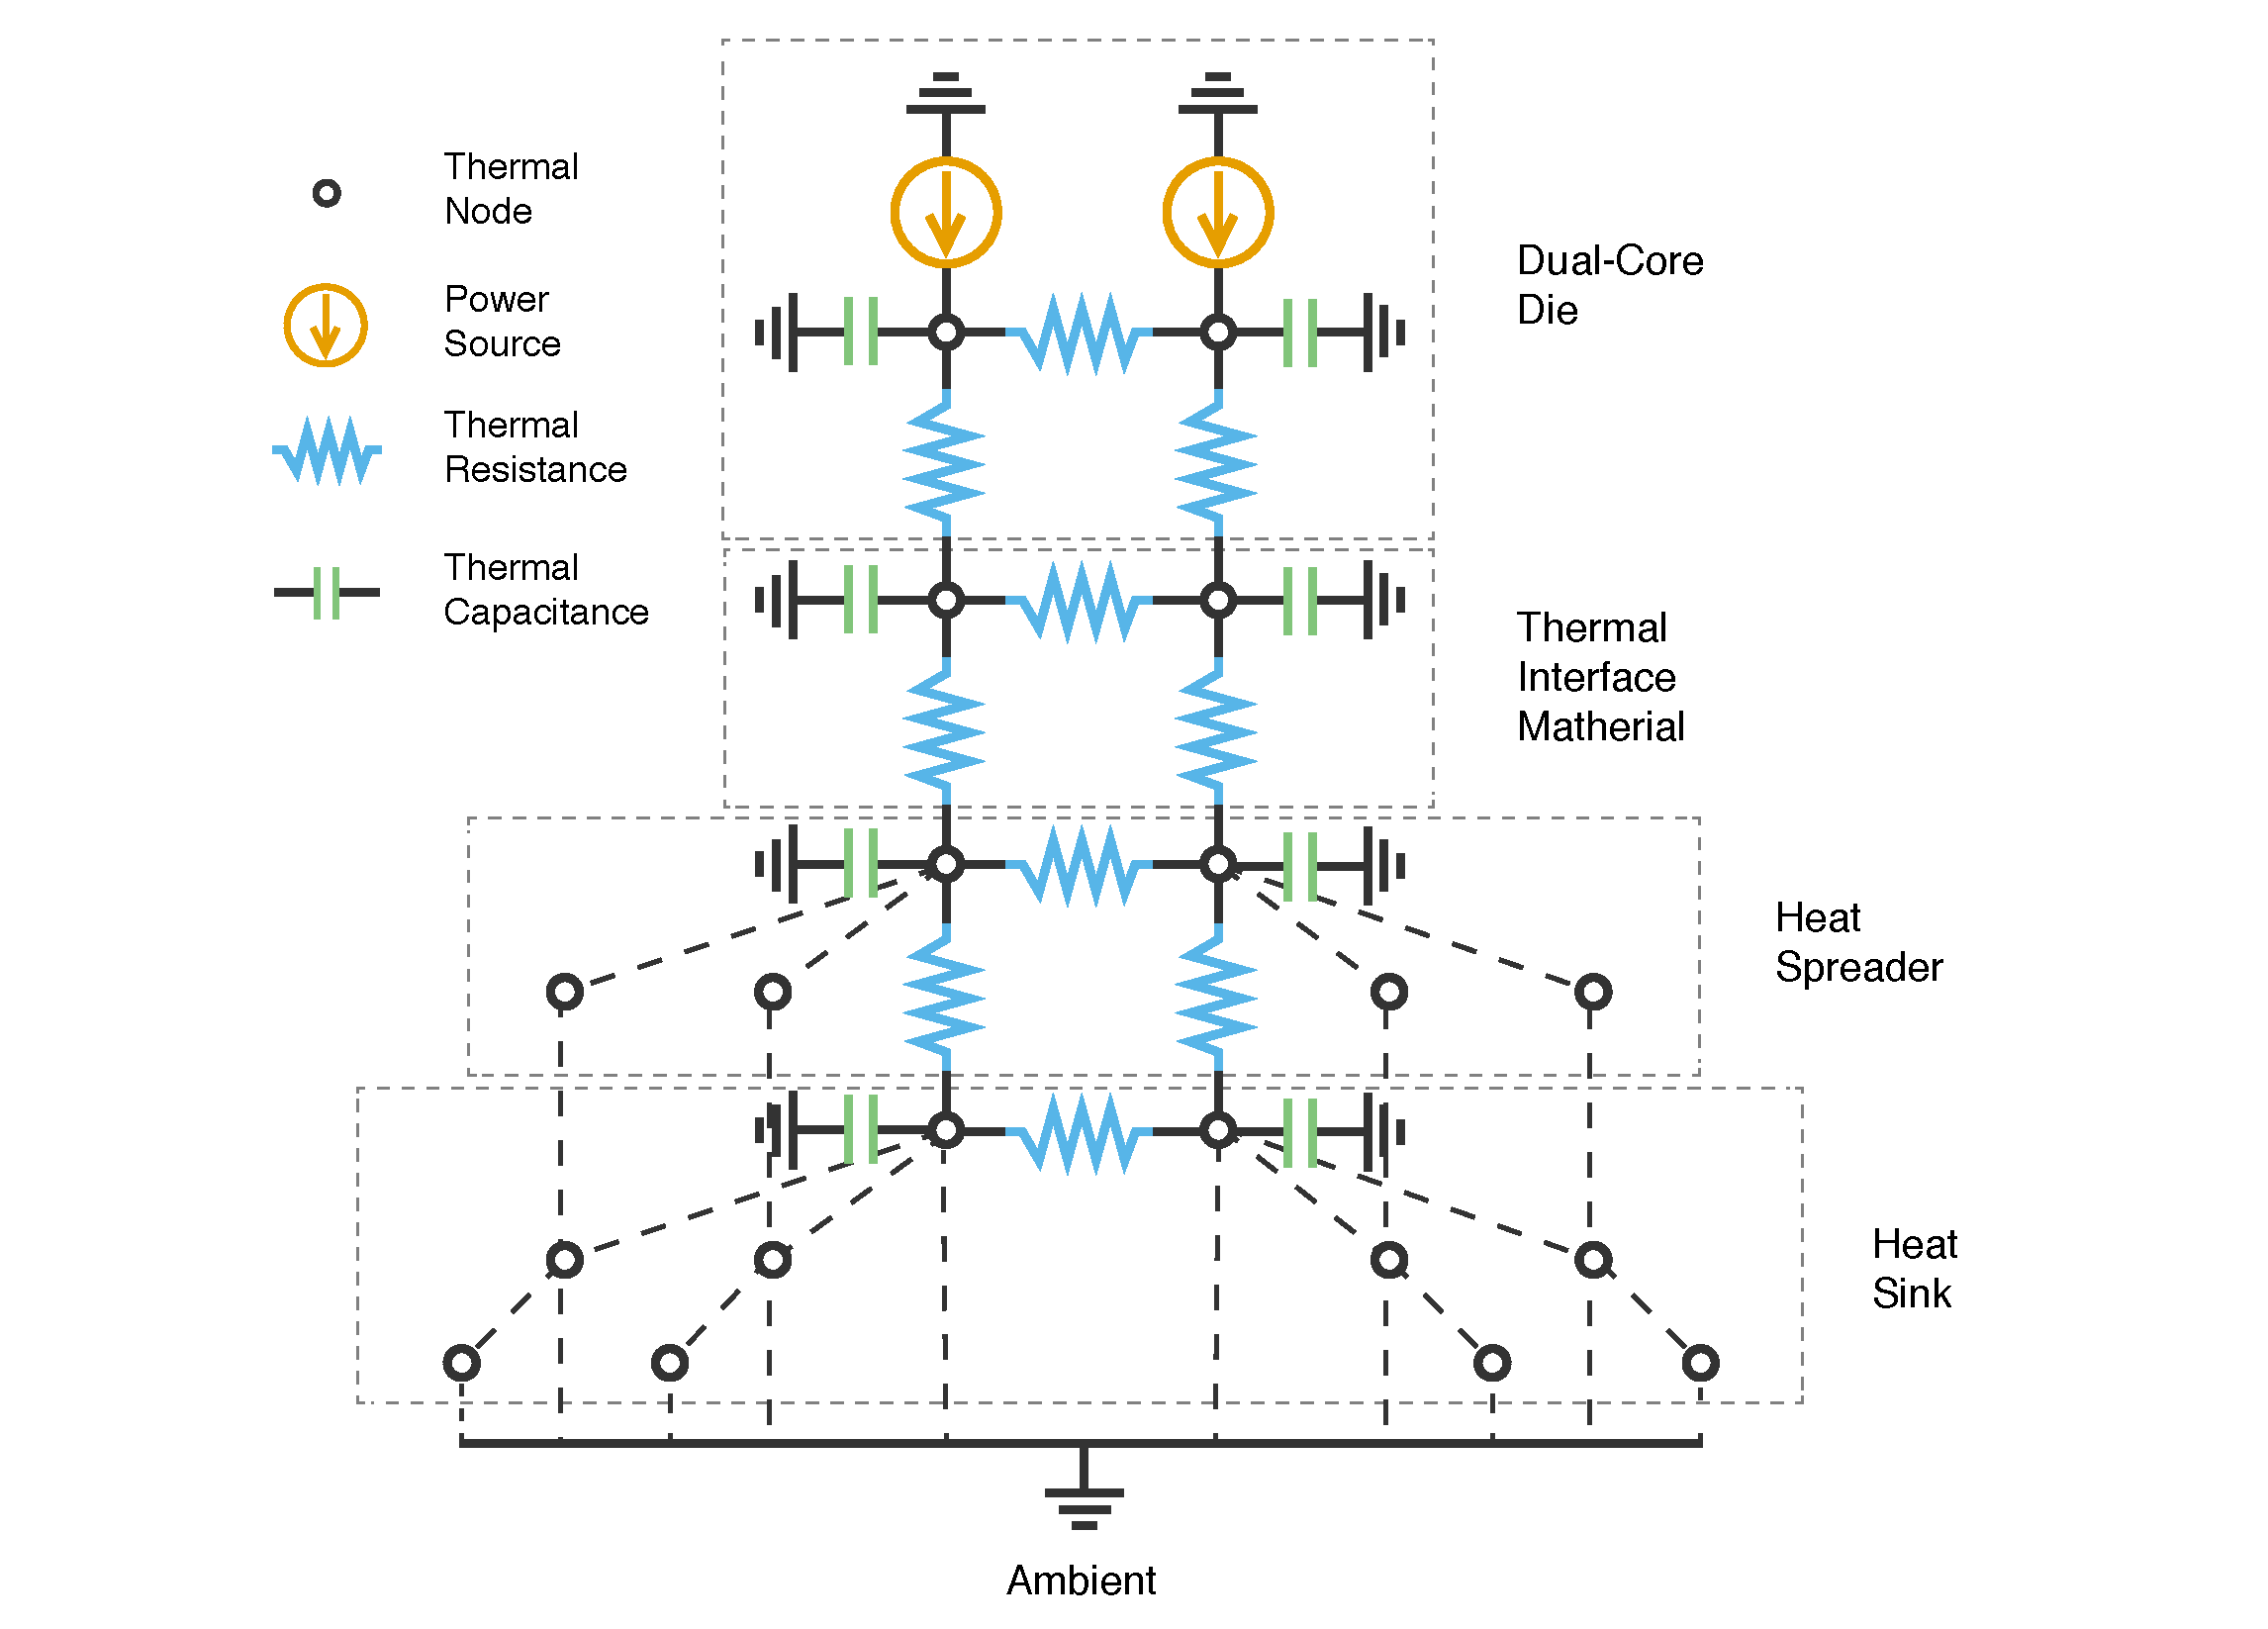
\includegraphics[width=\linewidth]{assets/circuit.pdf}
  \vspace{-15pt}
  \caption{Equivalent RC thermal circuit.}
  \label{fig:circuit}
  \vspace{15pt}
\end{figure}
